%************************************************
\chapter{Validation regions}
\label{ch:VR}
%************************************************

In order to ensure the estimations of the backgrounds are robust, two validation regions (VRjet1 and VRjet23) are defined for the corresponding two signal regions (SRjet1 and SRjet23), to compare the backgrounds and the data.
There are three requirements for the validation regions:
\begin{itemize}
\item The signal contribution is small.
\item The validation region is orthogonal to the corresponding signal region.
\item The background composition is similar to the corresponding signal region.
\end{itemize}
The definitions of the two validation regions are summarized in table \ref{tab:VR_cuts}.

\begin{table}[htbp]
\begin{center}
\begin{tabular}{|c|c|c|}
\hline
Cut & VRjet1 & VRjet23 \\
\hline
\hline
$n_{\text{jets}}$               & 1                             & $[2,3]$ \\
$\Delta \eta_{ll}$              & $<1.5$                        & $-$ \\
$E_T^{\text{miss}}$ [GeV]       & \textcolor{red}{ $[70,100]$ } & $>100$ \\
$m_T$ [GeV]                     & $>140$                        & \textcolor{red}{$[65,120]$} \\
$m_{\text{eff}}$ [GeV]          & $\textcolor{red}{-}$          & $>240$ \\
$m_{lj(j)}$ [GeV]               & \textcolor{red}{$>130$}       & \textcolor{red}{$>130$} \\
$m_{T2}$ [GeV]                  & $\textcolor{red}{-}$          & $\textcolor{red}{-}$ \\
\hline
\end{tabular}
\caption{The definition of the two validation regions on top of the pre-selections in section \ref{sec:SR_pre-selection}. The values in red colour represent different cuts compared to the signal regions.}
\label{tab:VR_cuts}
\end{center}
\end{table}

For the VRjet1, the validation region is obtained by reversing the $E_T^{\text{miss}}$ cut compared to the signal region.
This can ensure that the validation region is orthogonal to the SRjet1.
The lower cut of $E_T^{\text{miss}}$ is optimized to 70 GeV.
Such a similar background composition is obtained compared with the SRjet1.
The cut on $m_{lj}$ is reversed and relaxed, in order to reduce the signal contribution and increase the statistics.
The cuts of $m_{\text{eff}}$ and $m_{T2}$ are also removed to increase the statistics.

For the VRjet23, the validation region is obtained by reversing the $m_T$ cut.
This can ensure that the validation region is orthogonal to the SRjet23.
The cut is optimized to 65 GeV to have a similar background composition.
The cut on $m_{ljj}$ is reversed to reduce the signal contribution.
To increase the statistics, the $m_{T2}$ cut is removed.

The fractions of signal contribution at different mass points are shown in figure \ref{fig:signal_contribution_VR}. The signal contributions are below 12\% and 10\% for VRjet1 and VRjet23 respectively.
Figures \ref{fig:background composition_1} and \ref{fig:background composition_2} show the background composition in the validation regions and in the corresponding signal regions.
The background compositions of the validation regions are similar compared with their corresponding signal regions.
Table \ref{tab:VR_yields} shows the expected number of events in each background and the observed number of events in data.
The comparisons of some variable distributions between the background and the data are also shown in figures \ref{fig:VRjet1_plot} and \ref{fig:VRjet23_plot} for VRjet1 and VRjet23 respectively.
The estimated background and the data agree with each other within the uncertainties.

\begin{figure}[htbp]
\centering
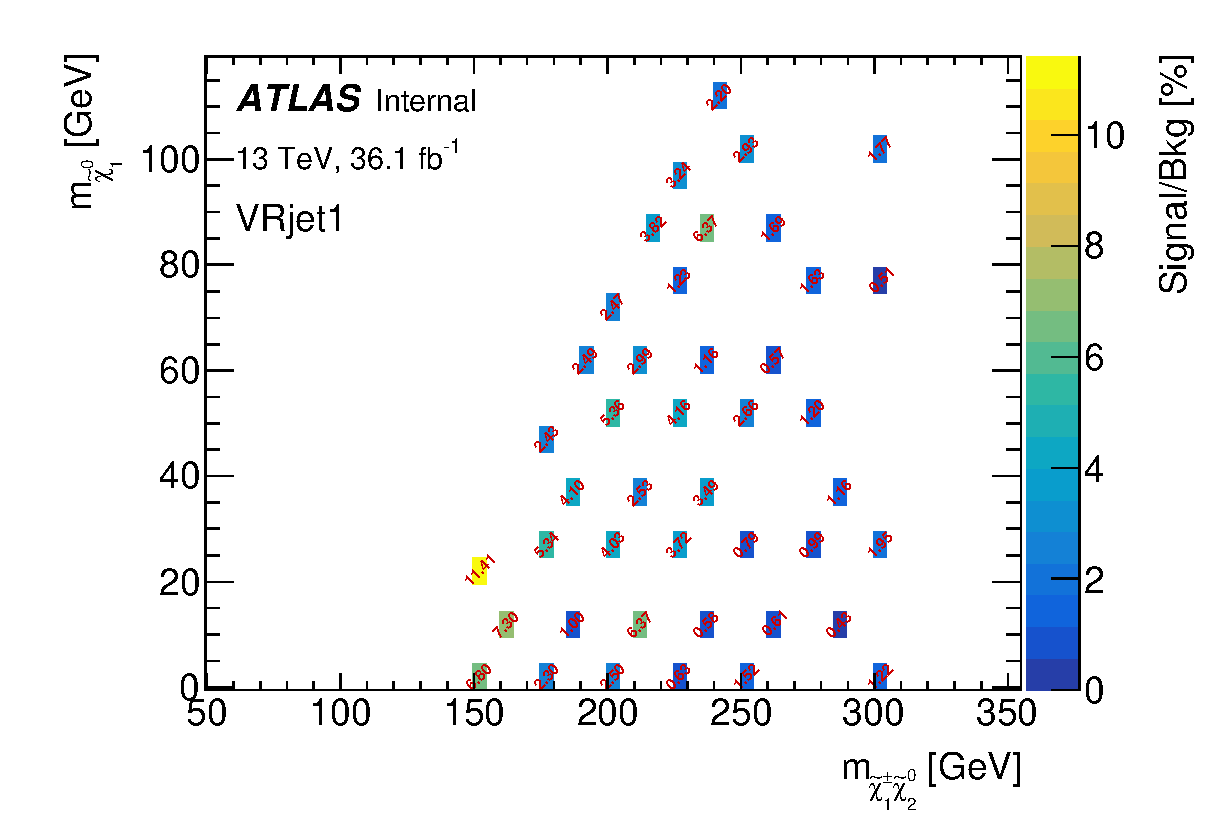
\includegraphics[width=0.45\textwidth]{data/plot/VR/SignalContamination_VRjet1.eps}
\includegraphics[width=0.45\textwidth]{data/plot/VR/SignalContamination_VRjet23.eps}
\caption{Fractions of signal contribution are shown for the VRjet1 (left) and VRjet23 (right).}
\label{fig:signal_contribution_VR}
\end{figure}

\begin{figure}[htbp]
\centering
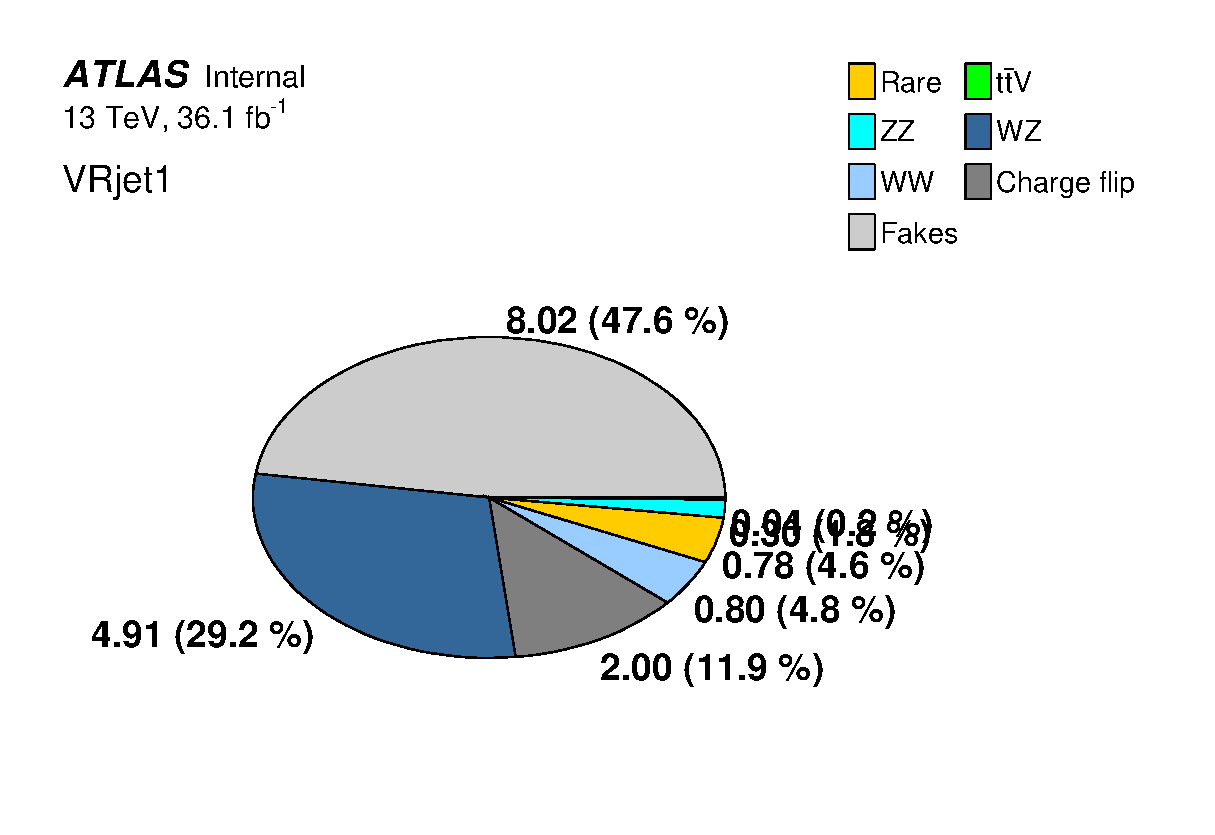
\includegraphics[width=0.45\textwidth]{data/plot/VR/BkgComposition_VRjet1.eps}
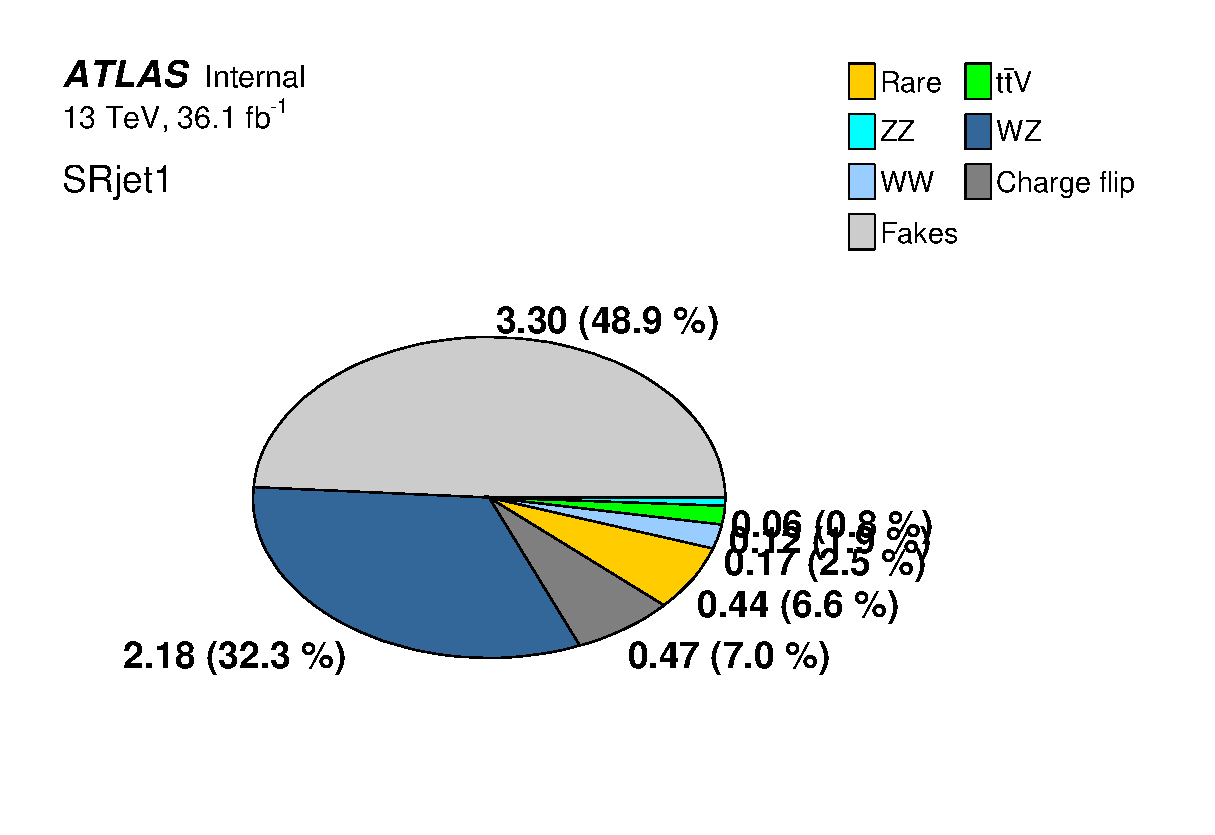
\includegraphics[width=0.45\textwidth]{data/plot/VR/BkgComposition_SRjet1.eps}
\caption{Background composition in the VRjet1 (left) and SRjet1 (right).}
\label{fig:background composition_1}
\end{figure}

\begin{figure}[htbp]
\centering
\includegraphics[width=0.45\textwidth]{data/plot/VR/BkgComposition_VRjet23.eps}
\includegraphics[width=0.45\textwidth]{data/plot/VR/BkgComposition_SRjet23.eps}
\caption{Background composition in the VRjet23 (left) and SRjet23 (right).}
\label{fig:background composition_2}
\end{figure}

\begin{table}[htbp]
\begin{center}
\begin{tabular}{|l|c|c|}
\hline
\hline
Process & VRjet1 & VRjet23 \\
\hline
\hline
Rare        & $0.775\pm 0.389^{+0.661}_{-0.362}$ & $2.469 \pm 0.674^{+0.998} _{-0.899}$ \\
$t\bar{t}V$ & $0.039\pm 0.013^{+0.018}_{-0.012}$ & $0.959 \pm 0.082^{+0.152} _{-0.146}$ \\
ZZ          & $0.298\pm 0.060^{+0.089}_{-0.063}$ & $0.247 \pm 0.045^{+0.113} _{-0.047}$ \\
WZ          & $4.909\pm 0.530^{+0.960}_{-0.899}$ & $19.325\pm 0.643^{+4.393} _{-4.346}$ \\
WW          & $0.801\pm 0.051^{+0.123}_{-0.060}$ & $10.477\pm 0.176^{+0.796} _{-0.726}$ \\
Charge flip & $1.997\pm 0.128^{+0.260}_{-0.260}$ & $2.065 \pm 0.085^{+0.166} _{-0.166}$ \\
Fakes       & $8.021\pm 1.390^{+5.806}_{-5.806}$ & $19.990\pm 2.013^{+13.461}_{-13.461}$ \\
\hline
Total BG      & $16.839\pm 1.545^{+5.915}_{-5.912}$ & $55.534\pm 2.228^{+14.396}_{-14.332}$ \\
\hline
\hline
Data        & $17$ & $54$ \\
\hline
\hline
\end{tabular}
\caption{The expected number of background events and the observed number of data events in the VRjet1 (the second column) and VRjet23 (the third column). The uncertainties include the statistical and systematic uncertainties.}
\label{tab:VR_yields}
\end{center}
\end{table}

\begin{figure}[htbp]
\centering
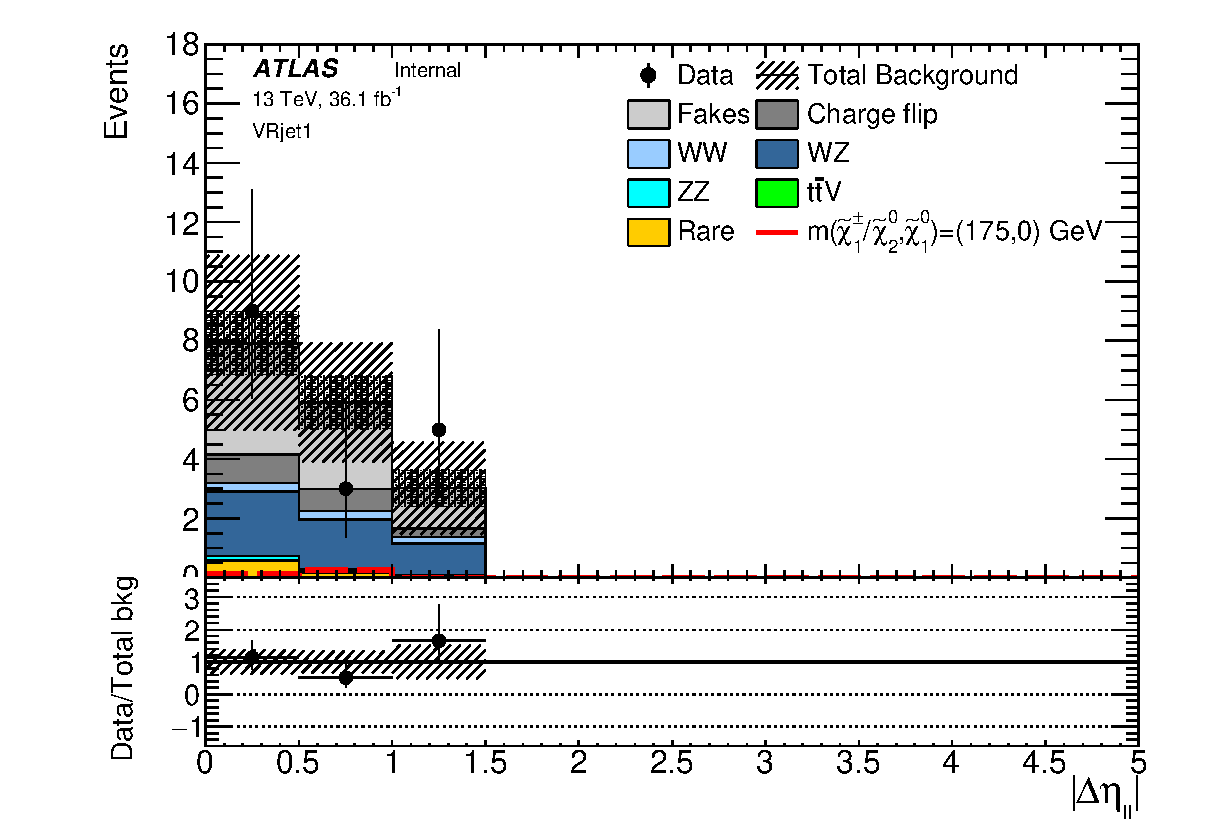
\includegraphics[width=0.47\textwidth]{data/plot/VR/all_DEtall_VRjet1.eps}
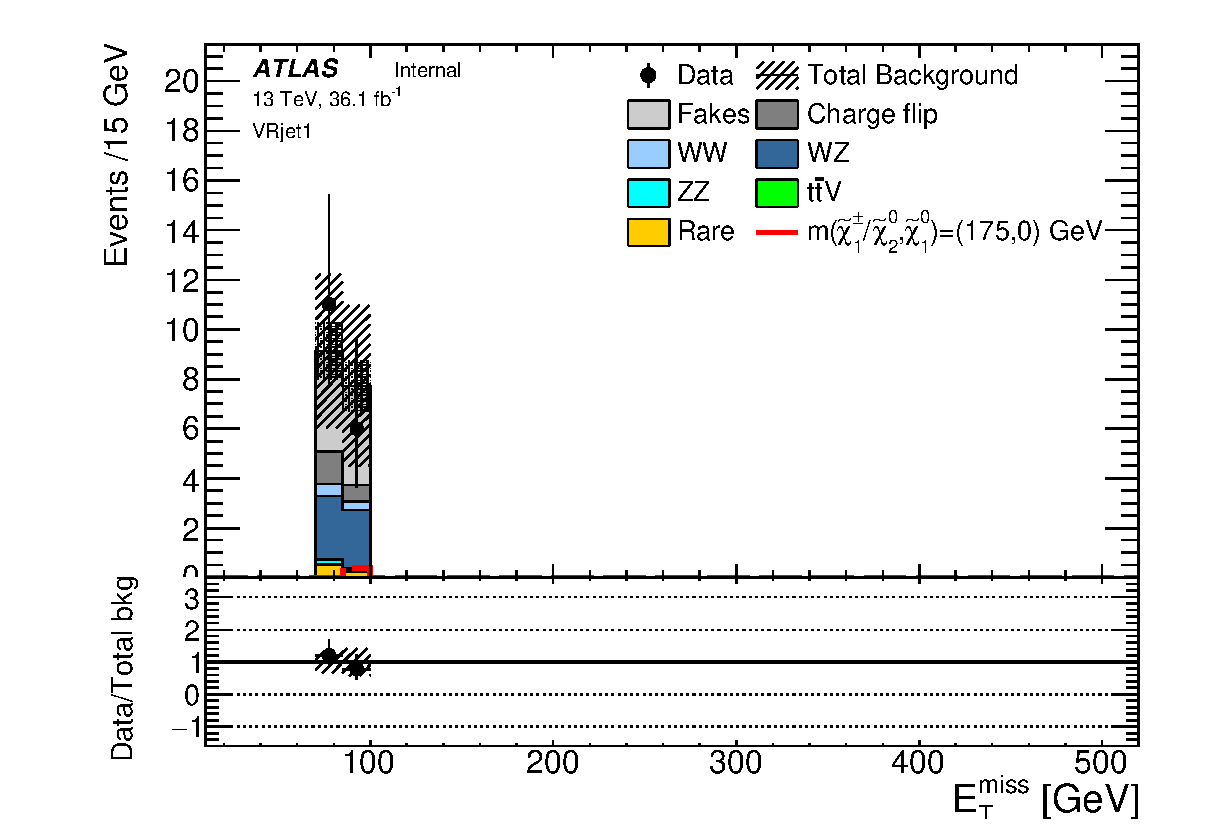
\includegraphics[width=0.47\textwidth]{data/plot/VR/all_Met_VRjet1.eps} \\
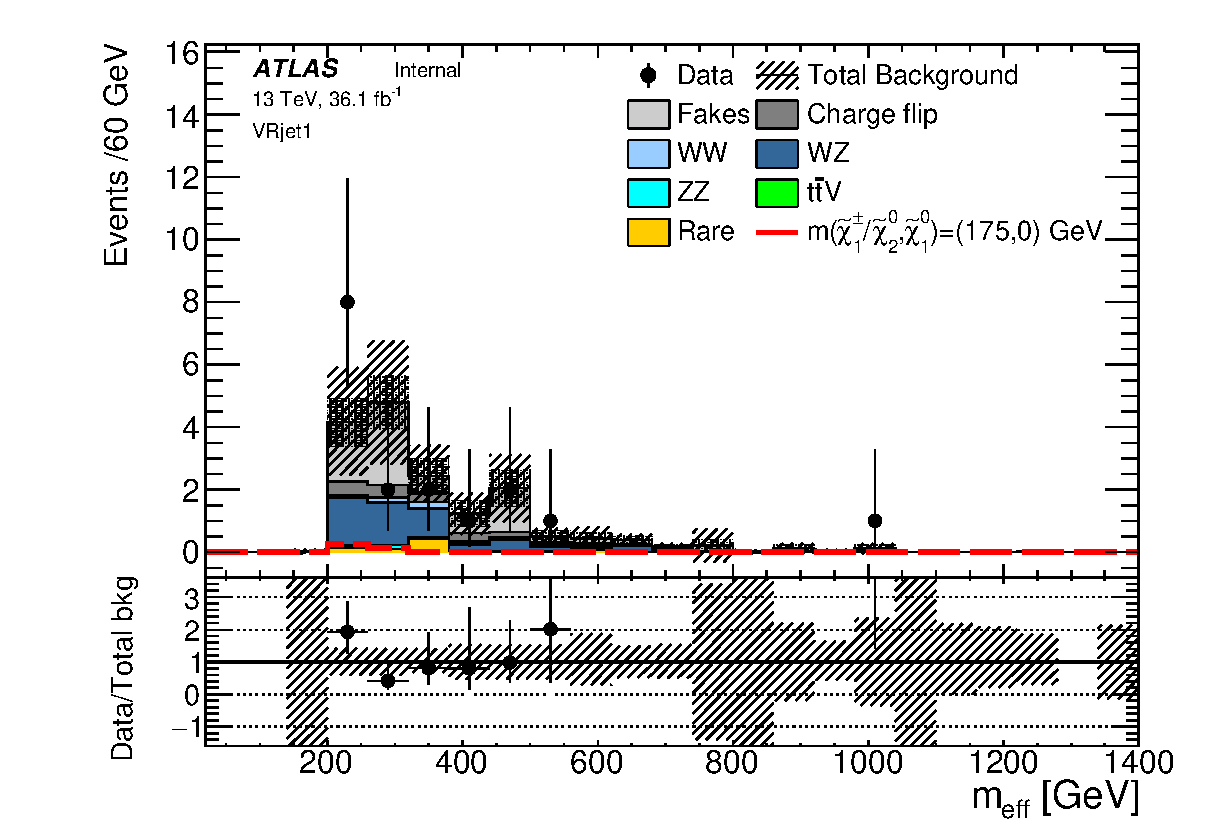
\includegraphics[width=0.47\textwidth]{data/plot/VR/all_Meff_VRjet1.eps}
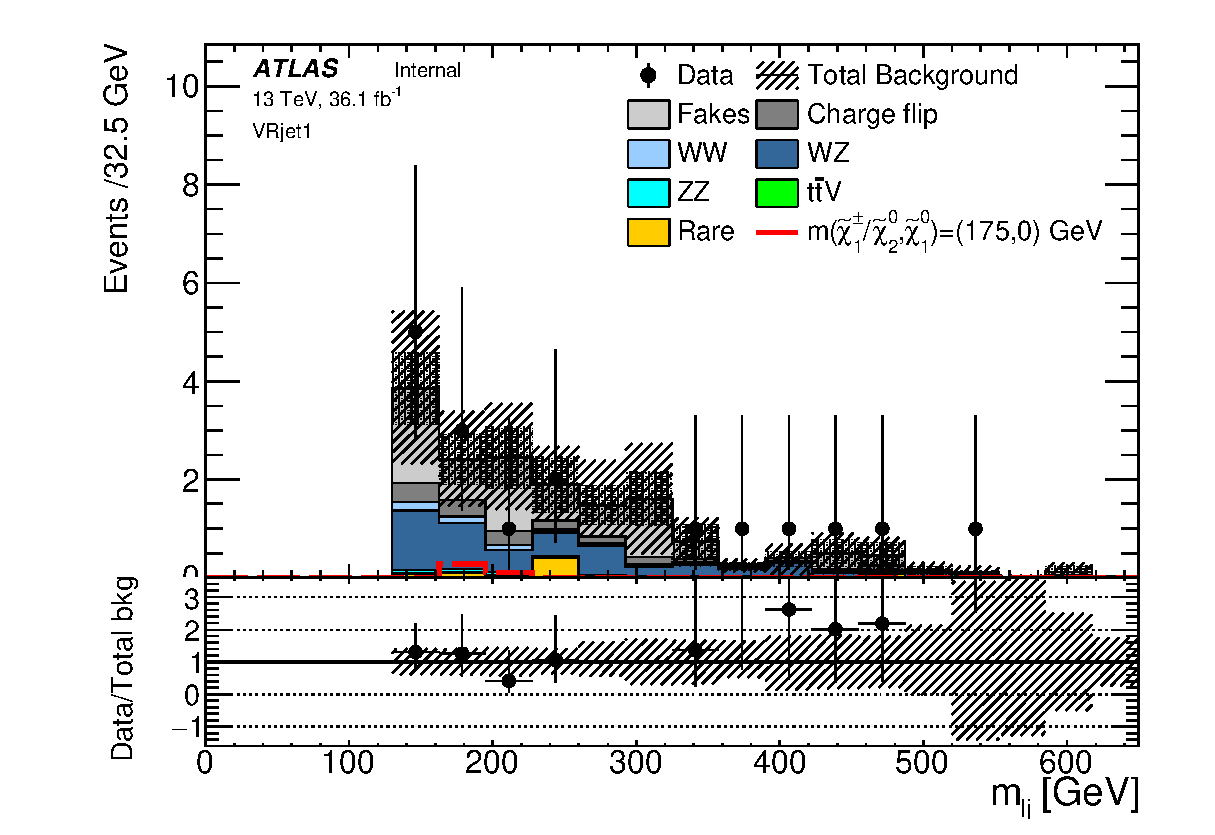
\includegraphics[width=0.47\textwidth]{data/plot/VR/all_Mlj_VRjet1.eps} \\
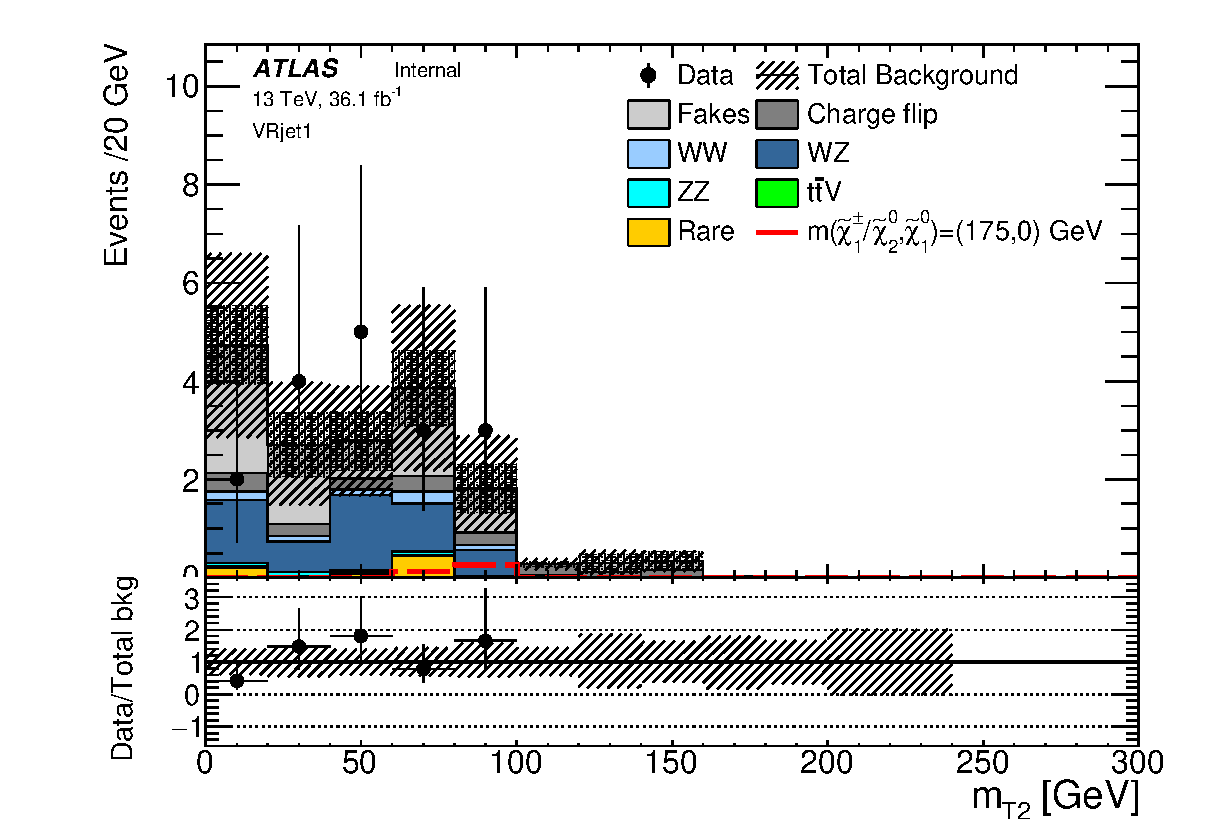
\includegraphics[width=0.47\textwidth]{data/plot/VR/all_Mt2_VRjet1.eps}
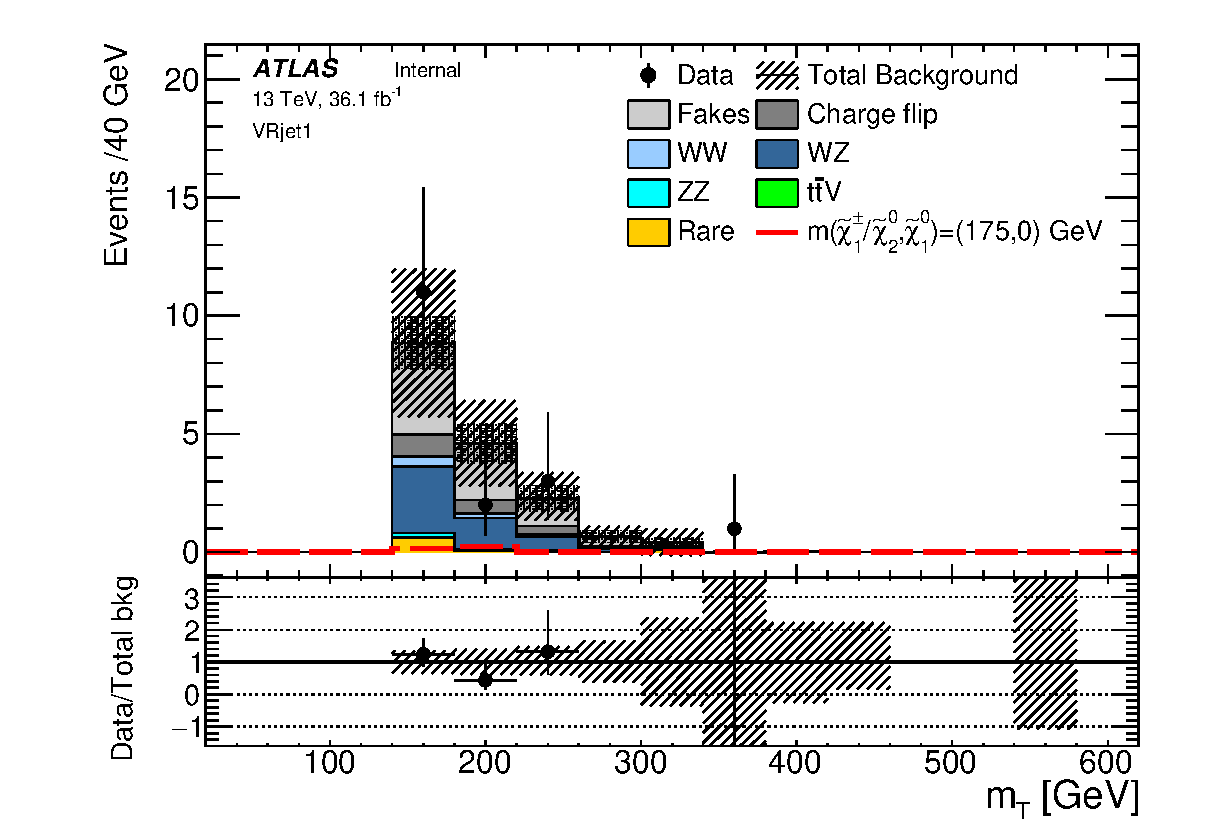
\includegraphics[width=0.47\textwidth]{data/plot/VR/all_Mt_VRjet1.eps} \\
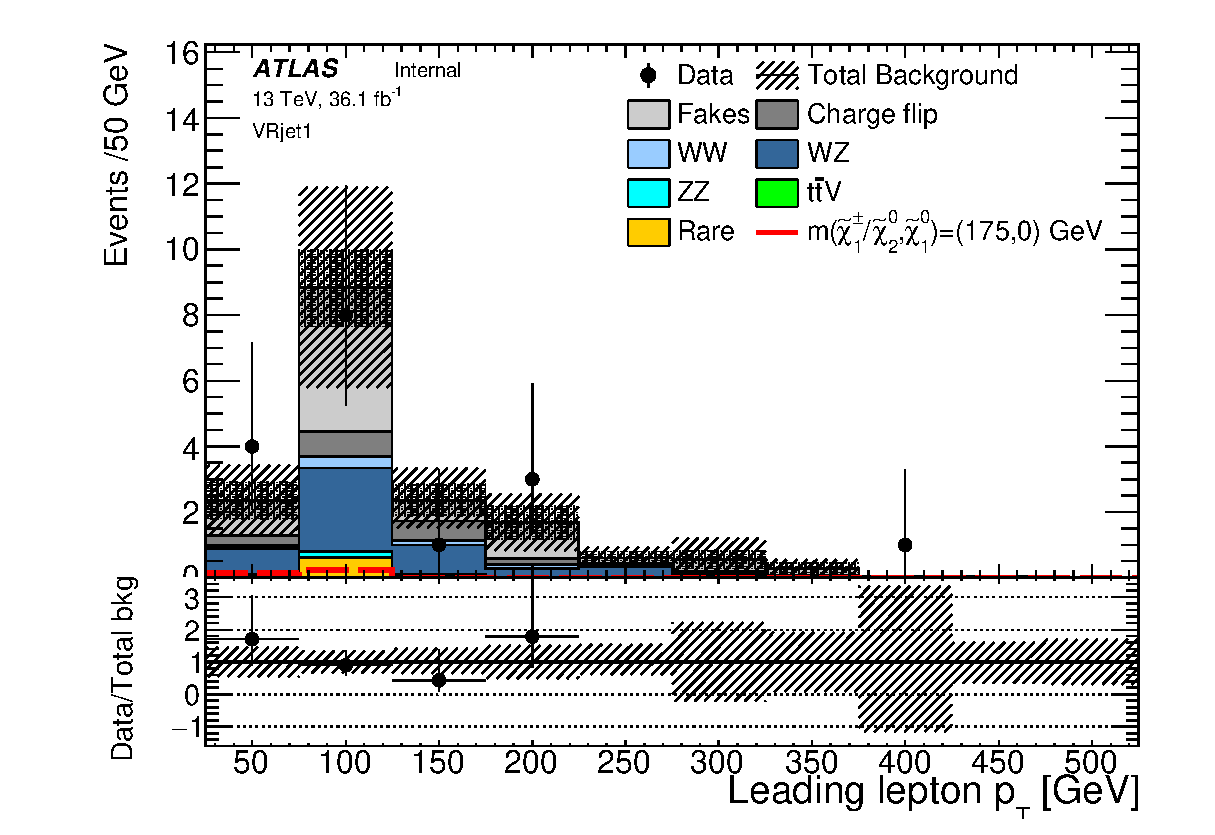
\includegraphics[width=0.47\textwidth]{data/plot/VR/all_PtLep_VRjet1.eps}
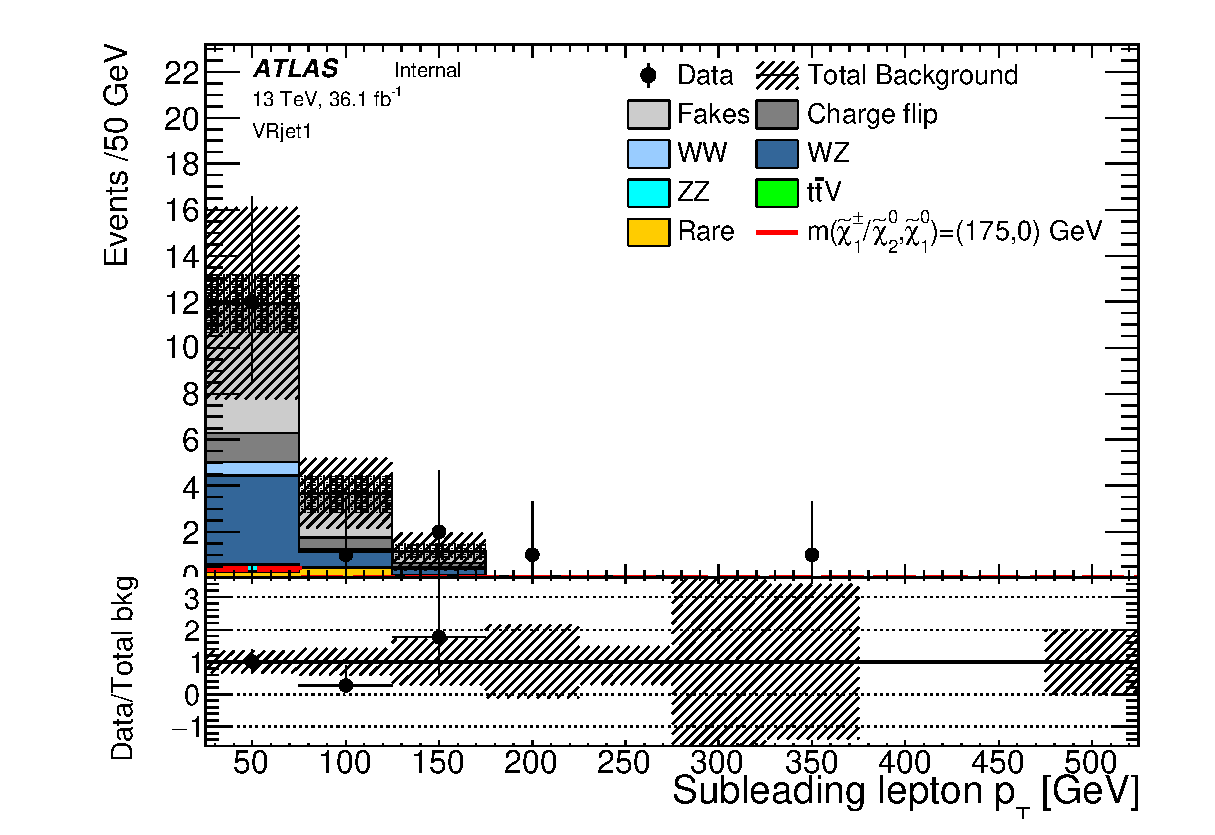
\includegraphics[width=0.47\textwidth]{data/plot/VR/all_PtSublep_VRjet1.eps} \\
\includegraphics[width=0.47\textwidth]{data/plot/VR/all_Njets_VRjet1.eps}
\caption{Distributions of the variables in the VRjet1 for the background estimation and the data are shown. A signal at a mass point ($m_{\tilde{\chi}_1^\pm , \tilde{\chi}_2^0}$,$m_{\tilde{\chi}_1^0}$) = (175,0) is also shown. The internal shaded area refers to the statistical uncertainties, while the external shaded area refers to the total uncertainty.}
\label{fig:VRjet1_plot}
\end{figure}

\begin{figure}[htbp]
\centering
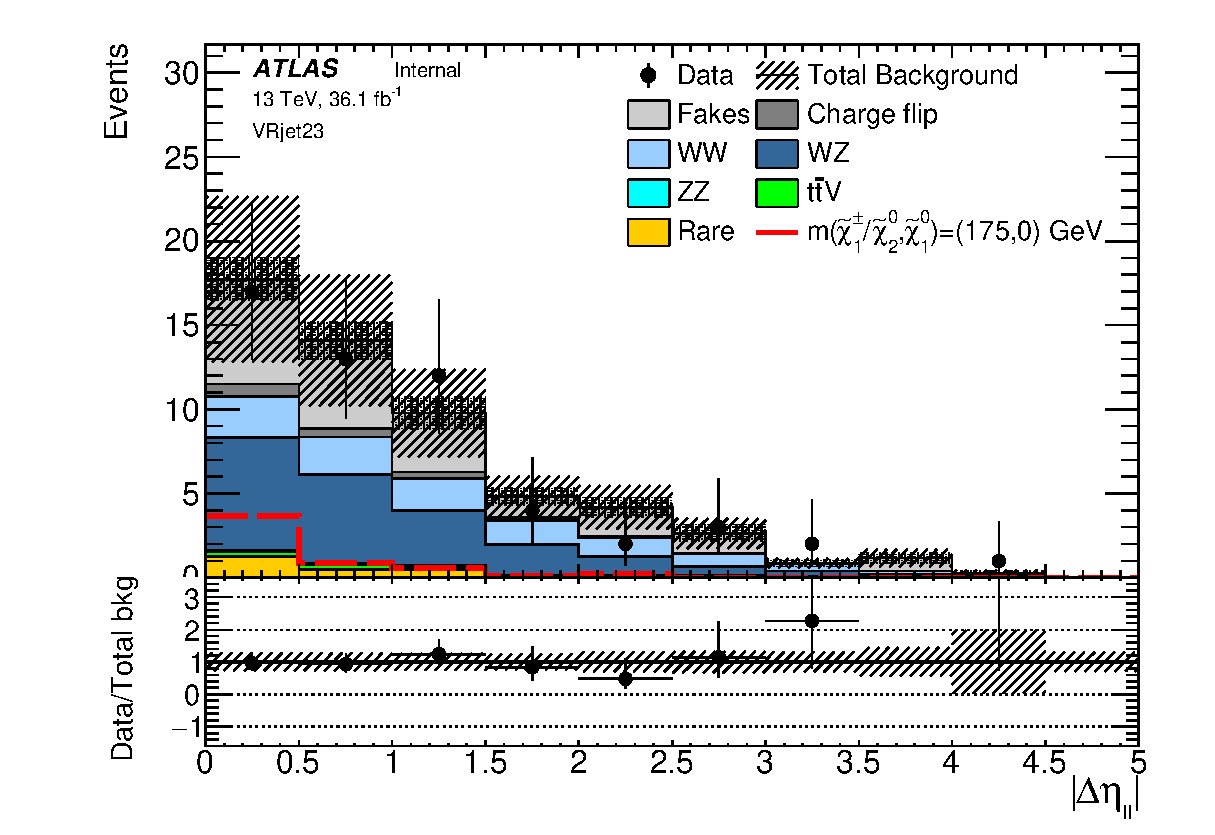
\includegraphics[width=0.47\textwidth]{data/plot/VR/all_DEtall_VRjet23.eps}
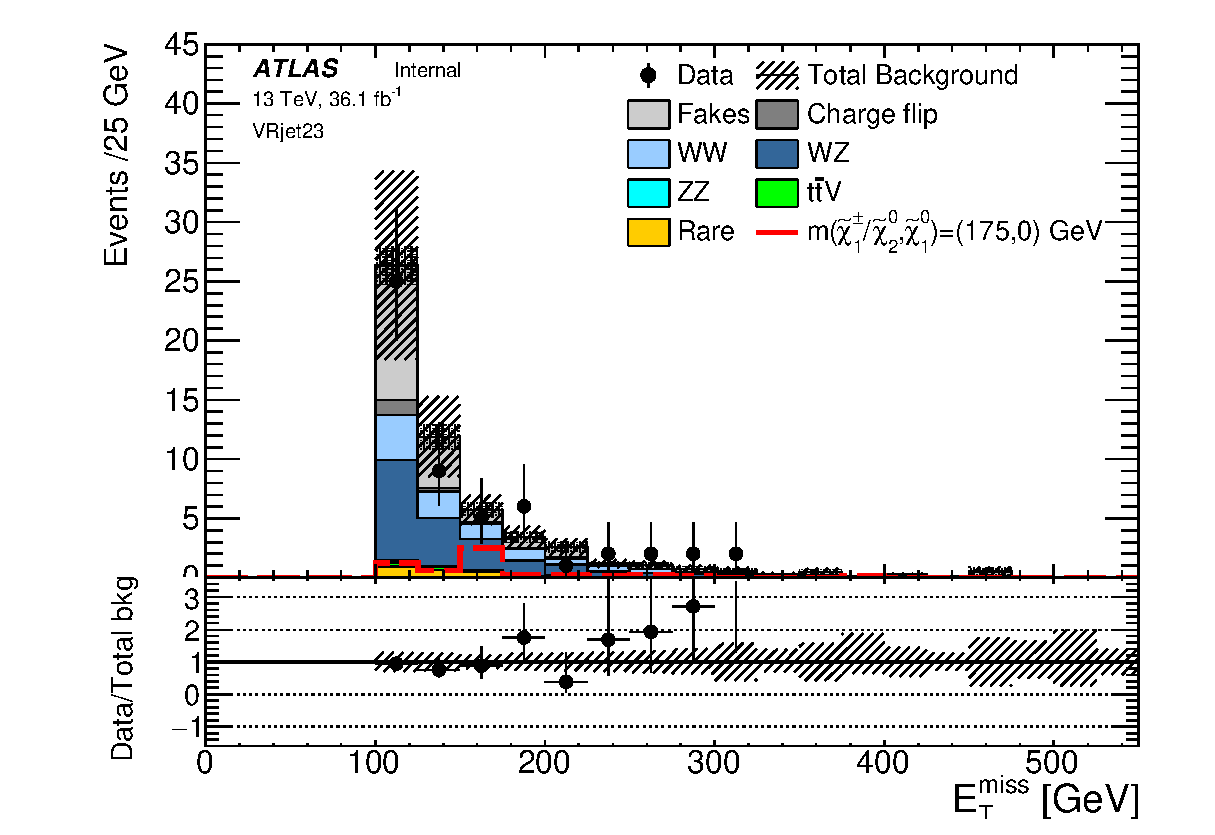
\includegraphics[width=0.47\textwidth]{data/plot/VR/all_Met_VRjet23.eps} \\
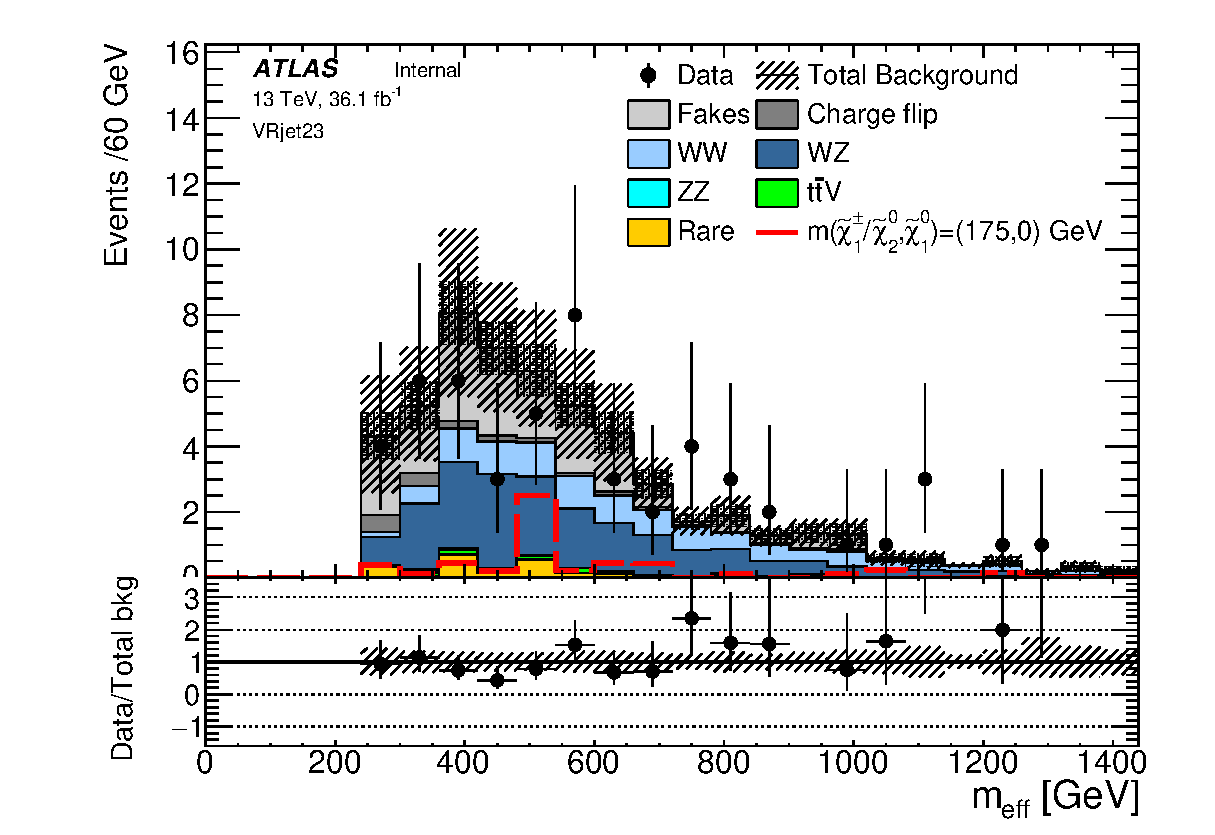
\includegraphics[width=0.47\textwidth]{data/plot/VR/all_Meff_VRjet23.eps}
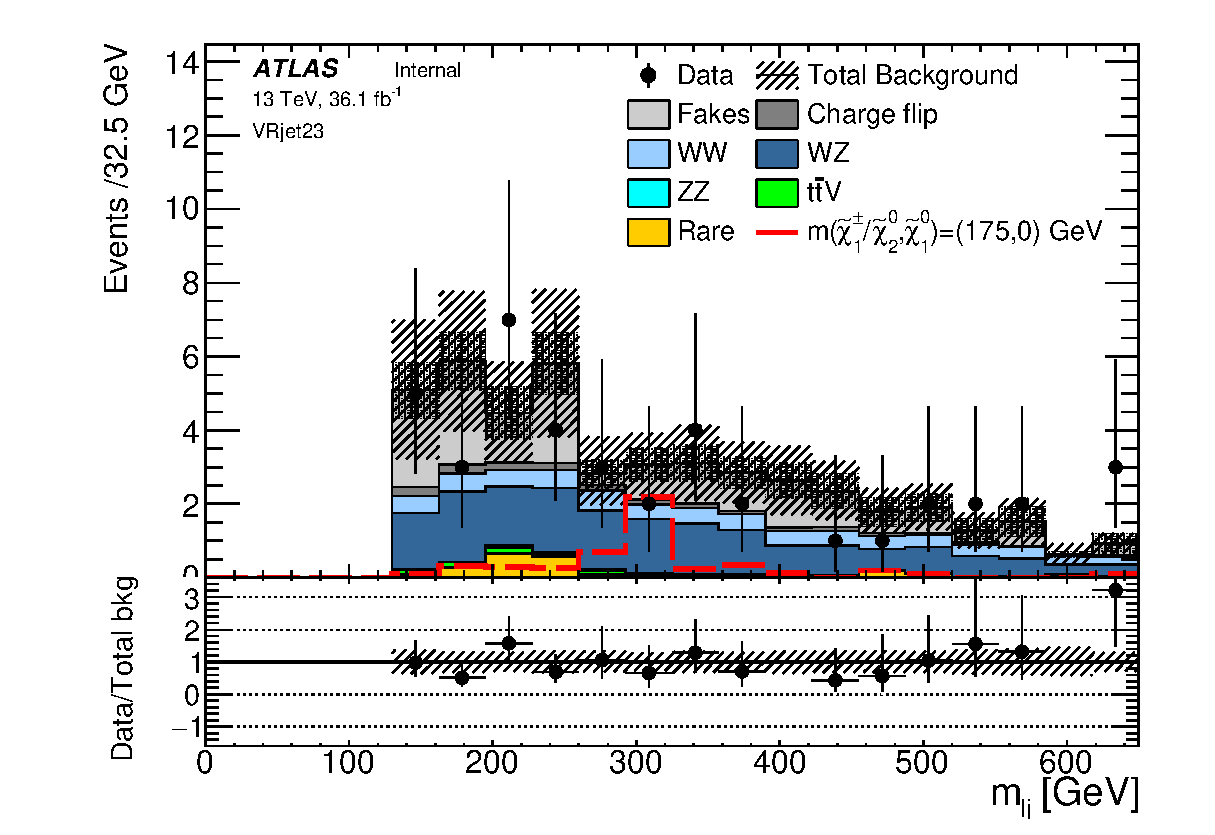
\includegraphics[width=0.47\textwidth]{data/plot/VR/all_Mlj_VRjet23.eps} \\
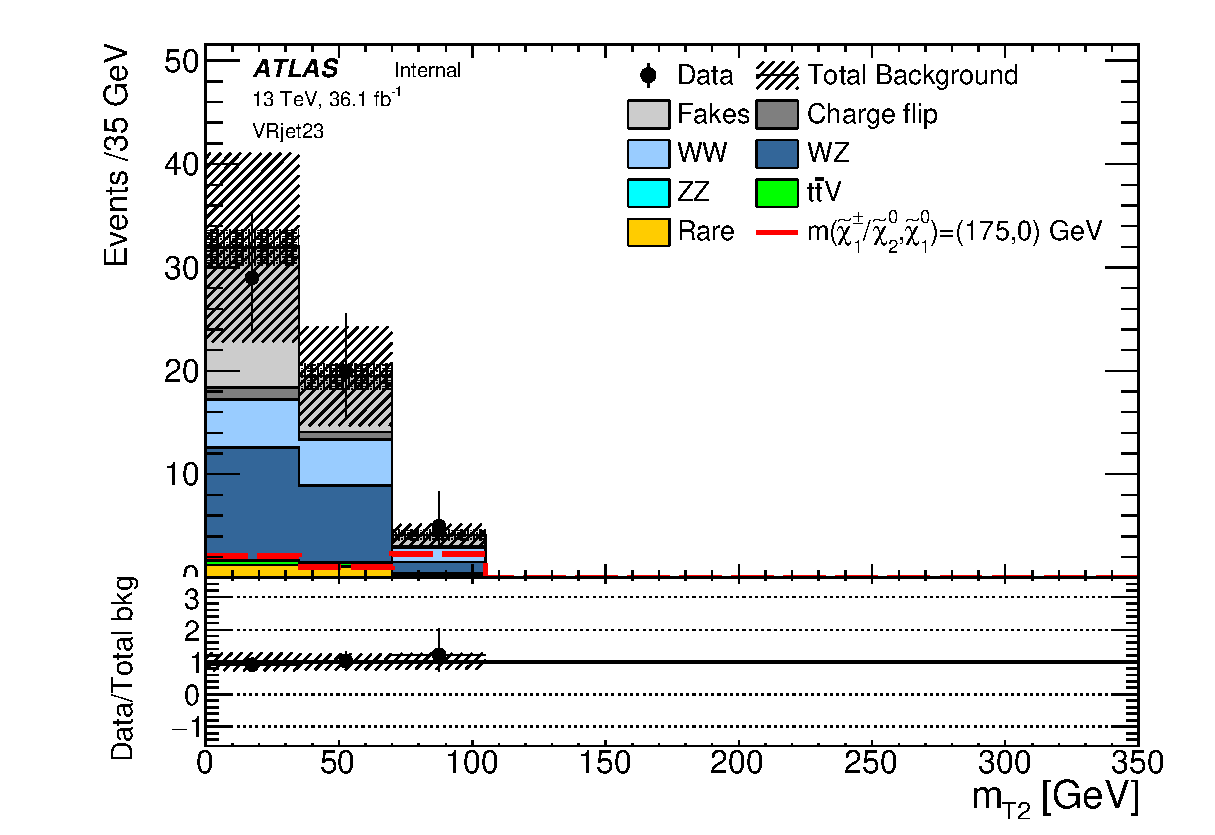
\includegraphics[width=0.47\textwidth]{data/plot/VR/all_Mt2_VRjet23.eps}
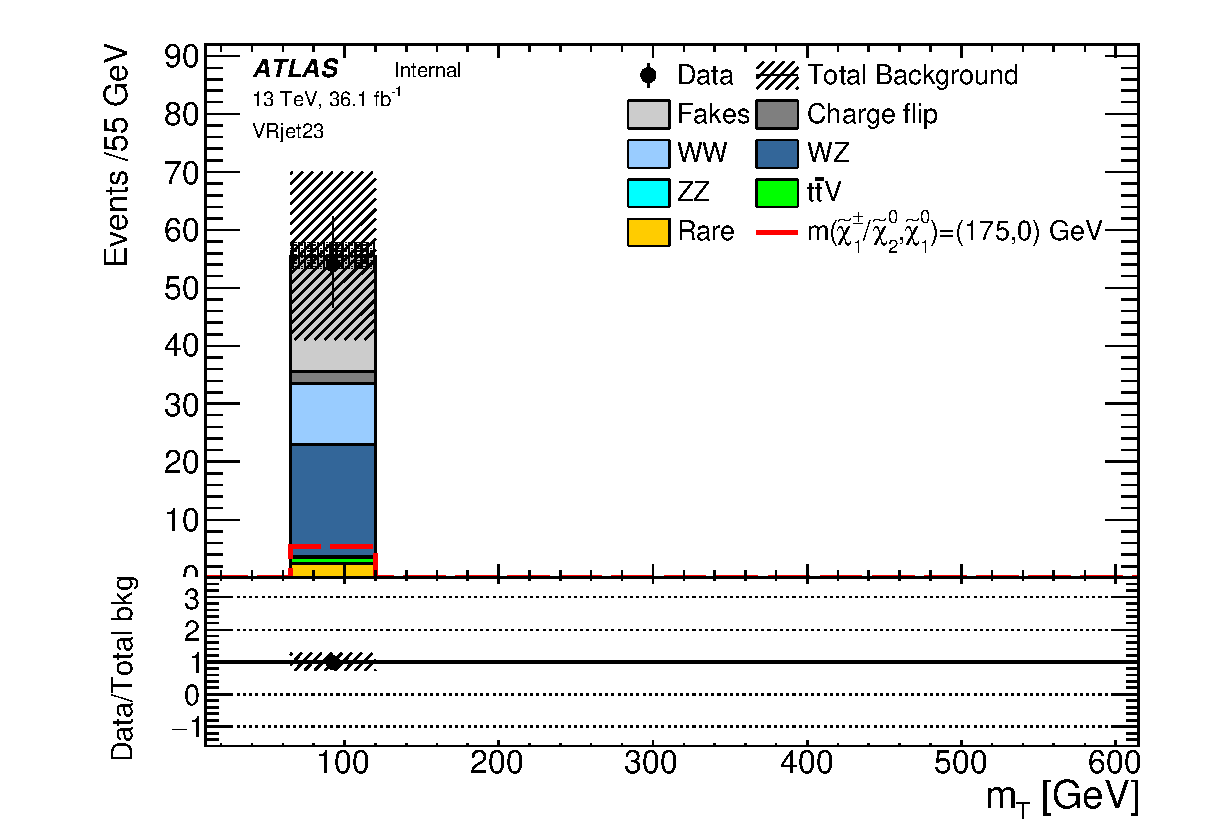
\includegraphics[width=0.47\textwidth]{data/plot/VR/all_Mt_VRjet23.eps} \\
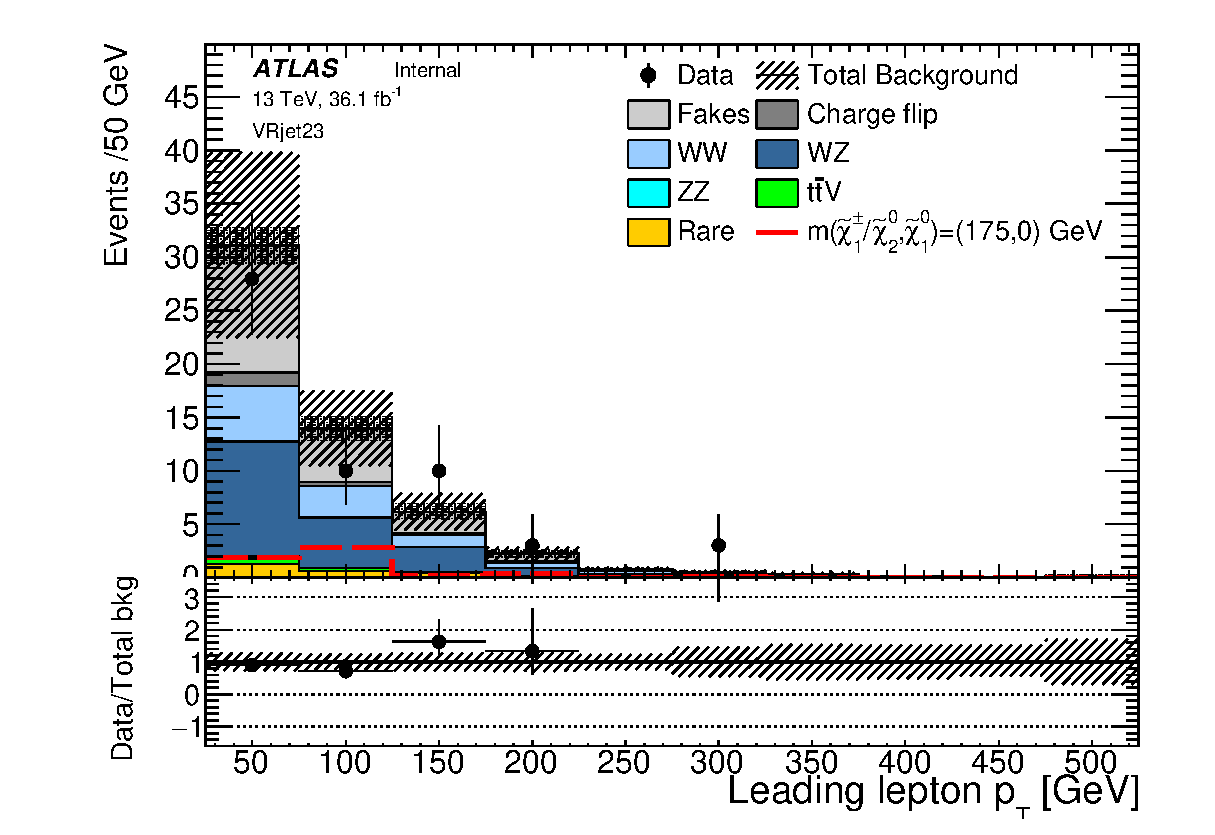
\includegraphics[width=0.47\textwidth]{data/plot/VR/all_PtLep_VRjet23.eps}
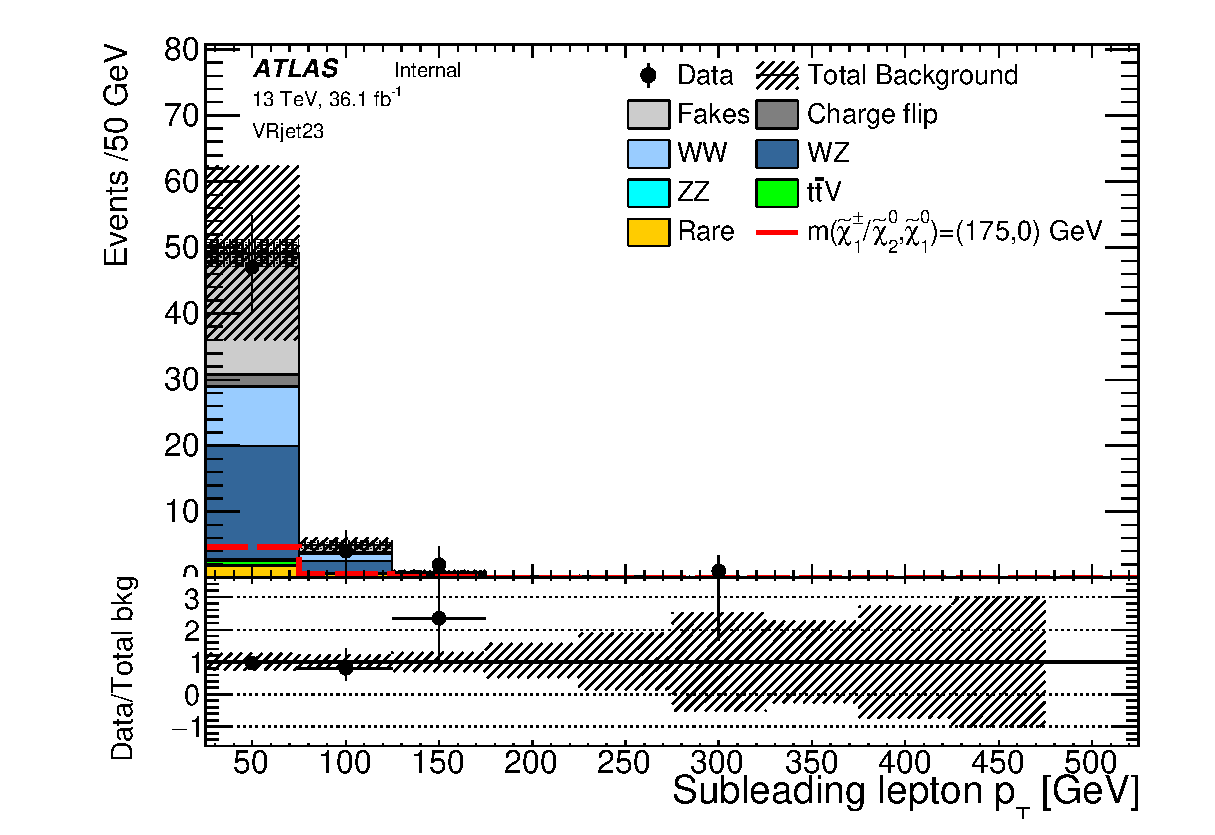
\includegraphics[width=0.47\textwidth]{data/plot/VR/all_PtSublep_VRjet23.eps} \\
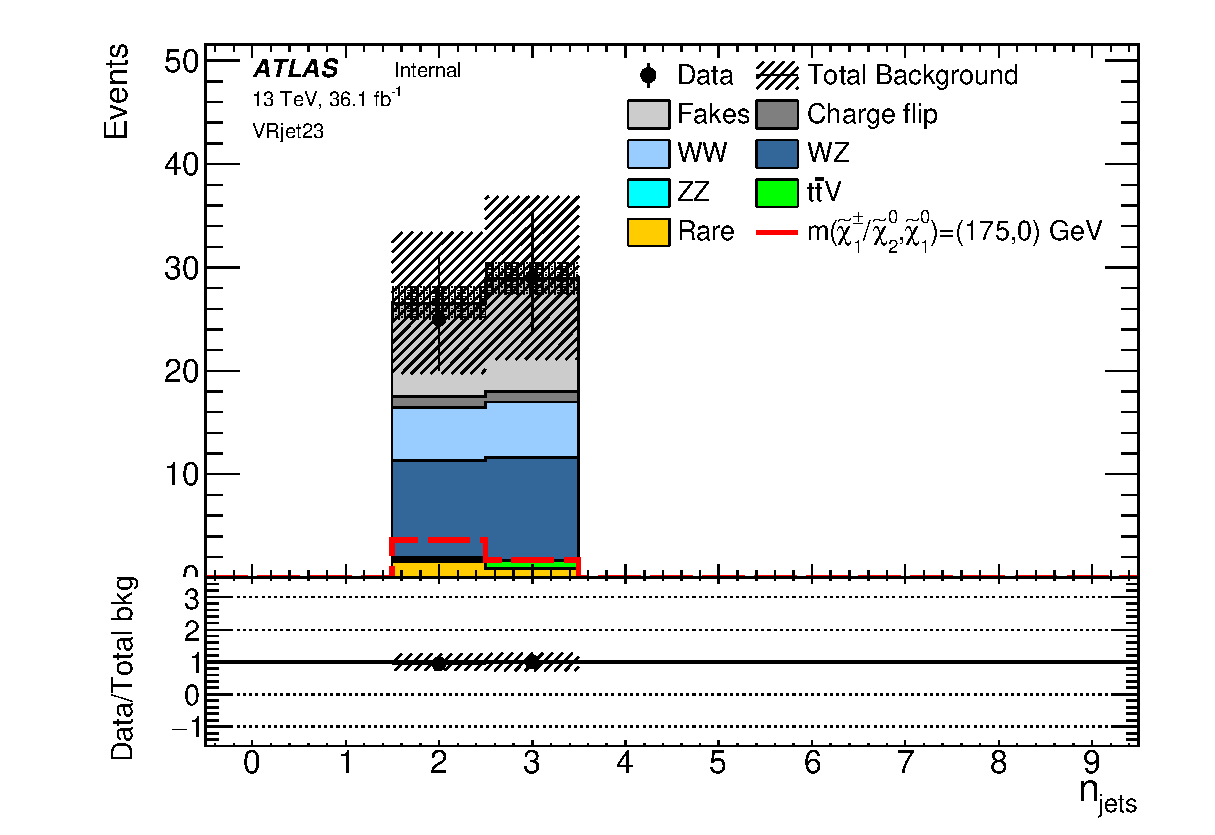
\includegraphics[width=0.47\textwidth]{data/plot/VR/all_Njets_VRjet23.eps}
\caption{Distributions of the variables in the VRjet23 for the background estimation and the data are shown. A signal at a mass point ($m_{\tilde{\chi}_1^\pm , \tilde{\chi}_2^0}$,$m_{\tilde{\chi}_1^0}$) = (175,0) is also shown. The internal shaded area refers to the statistical uncertainties, while the external shaded area refers to the total uncertainty.}
\label{fig:VRjet23_plot}
\end{figure}
